%%
%% IEEE Transactions on Multimedia (TMM)
%% End-to-End Subtitle Recognition & Chinese-Japanese Translation
%% with Speech Synthesis in Short Dramas
%%
%% TMM uses IEEEtran (journal) class. Compile with XeLaTeX + bibtex
%% (XeLaTeX is required for the Chinese/Japanese characters in the
%% qualitative-examples table; see the xeCJK package below).
%%  xelatex main && bibtex main && xelatex main && xelatex main
%%
%% Note: TMM review submissions use double-column journal style.
%%  Submission (review): \documentclass[journal]{IEEEtran}
%%  Camera-ready:     \documentclass[journal]{IEEEtran}
%%
\documentclass[journal]{IEEEtran}

\usepackage{cite}
\usepackage{amsmath,amssymb,amsfonts}
\usepackage{graphicx}
\usepackage{booktabs}
\usepackage{multirow}
\usepackage{algorithm}
\usepackage{algpseudocode}
\usepackage{url}
\usepackage{xcolor}
\usepackage{array}
\usepackage{pgfplots}
\pgfplotsset{compat=1.18}

% --- CJK support (Chinese source + Japanese translations in qualitative examples) ---
% REQUIRES the XeLaTeX compiler (Overleaf: Menu -> Compiler -> XeLaTeX).
% Noto Serif CJK SC covers both Chinese hanzi and Japanese kanji/kana and is
% available on Overleaf and full TeX Live installations.
\usepackage{xeCJK}
\setCJKmainfont{Noto Serif CJK SC}

\hyphenation{op-tical net-works semi-conduc-tor}

\begin{document}

\title{An End-to-End Multimodal System for Subtitle Recognition and Chinese--Japanese Translation with Speech Synthesis in Short Dramas}

\author{Qiming~Bao,
    Jing~An,
    Rui-Yang~Ju,
    Haofei~Chang,
    Jinhua~Su,
    Yanbing~Bai,
    Xin~Qu,
    and~Michael~Witbrock%
\thanks{Qiming Bao and Jing An contributed equally as joint first authors.}%
\thanks{Yanbing Bai and Jing An are corresponding authors.}%
\thanks{Q. Bao is with the University of Auckland, Auckland 1010, New Zealand (e-mail: qiming.bao@auckland.ac.nz).}%
\thanks{J. An and X. Qu are with the School of AI and Language Sciences, Beijing International Studies University, Beijing 100024, China (e-mail: jing.an@bisu.edu.cn; xin.qu@bisu.edu.cn).}%
\thanks{R.-Y. Ju is with the Graduate School of Informatics, Kyoto University, Kyoto 606-8501, Japan (e-mail: ju.ruiyang.65e@st.kyoto-u.ac.jp).}%
\thanks{H. Chang is with the School of Information, Renmin University of China, Beijing 100872, China (e-mail: hfchang@ruc.edu.cn).}%
\thanks{J. Su is with the Center for Applied Statistics, School of Statistics, Renmin University of China, Beijing 100872, China, and also with Simashuhui Ltd., Beijing 100086, China (e-mail: sujinhua@ruc.edu.cn).}%
\thanks{Y. Bai is with the Center for Applied Statistics, School of Statistics, Renmin University of China, Beijing 100872, China (e-mail: ybbai@ruc.edu.cn).}%
\thanks{M. Witbrock is with the School of Computer Science, University of Auckland, Auckland 1010, New Zealand (e-mail: m.witbrock@auckland.ac.nz).}%
\thanks{Manuscript received Month XX, 2026; revised Month XX, 2026.}}

\markboth{IEEE Transactions on Multimedia,~Vol.~XX, No.~X, Month~2026}%
{Bao \MakeLowercase{\textit{et al.}}: An End-to-End Multimodal System for Subtitle Recognition and Chinese--Japanese Translation with Speech Synthesis in Short Dramas}

\maketitle

\begin{abstract}
Chinese short-form drama (\emph{duanju}) has become a globally consumed multimedia format, creating industrial demand for automated subtitle localization spanning recognition, translation, and dubbing. This domain challenges existing subtitling tools: dialogue is fast-paced and colloquial, on-screen text and audio are weakly aligned, and character-specific proper nouns are dense. We propose an \emph{end-to-end multimodal subtitle processing system} performing visual subtitle recognition, audio transcription, neural machine translation, and zero-shot Japanese voice cloning, evaluated stage-by-stage on a manually annotated Chinese--Japanese short-drama corpus (79 episodes; 3{,}692 segments). For recognition, we compare eight OCR backbones against Whisper ASR and introduce a \emph{confidence-adaptive multimodal fusion} that gates between Whisper and Qwen3-VL OCR using segment-level log-probabilities, improving the composite recognition score by $+10.8\%$ over ASR-only. For translation, LoRA fine-tuning achieves cross-validated BLEU $15.70\pm4.42$ / COMET $0.843\pm0.026$ with Qwen3-VL-4B and BLEU $19.69\pm2.49$ / COMET $0.860\pm0.016$ with text-only Qwen3-8B, outperforming nine of eleven zero-shot baselines including all dedicated MT models and comparable multimodal VLMs; fine-tuning helps at every scale tested, with a 12B fine-tune setting the quality ceiling at BLEU $30.75\pm1.84$. Fusion benefits propagate downstream: it corrects $60\%$ of misrecognized proper nouns and recovers $+2.24$ chrF\texttt{++} (61\% of oracle) over ASR-only in direct end-to-end evaluation. For synthesis, we benchmark four zero-shot TTS systems; GPT-SoVITS achieves the best intelligibility among voice-cloning systems, and a blind five-rater listening study confirms it matches commercial EdgeTTS naturalness (MOS 3.08 vs.\ 3.12) while dominating perceived speaker similarity (45\% of votes). To our knowledge these results establish the first end-to-end multimodal benchmark for Chinese short-drama localization.
\end{abstract}

\begin{IEEEkeywords}
Subtitle recognition, subtitle translation, text-to-speech, Chinese short dramas, multimedia localization, multimodal fusion, vision-language models, large language models, zero-shot voice cloning.
\end{IEEEkeywords}

\IEEEpeerreviewmaketitle

%%
%% Introduction
%%
\section{Introduction}
\label{sec:introduction}
\IEEEPARstart{T}{he} global rise of Chinese short dramas (\textit{duanju})---3--15-minute episodes produced at industrial cadence and watched by hundreds of millions across China, North America, Southeast Asia, Japan, and Korea---has created strong demand for cross-lingual subtitling and dubbing.
Localization here is fundamentally a \emph{multimedia} task in which subtitle text, audio, and visual frame are tightly coupled; yet short dramas feature fast-paced, colloquial dialogue with on-screen text changing 2--5 times per second, so conventional pipelines that chain independent off-the-shelf recognition, translation, and synthesis components are ill-equipped for consistent end-to-end localization.

\textbf{Challenges in subtitle processing.}
Short-drama localization poses five coupled difficulties: (i) inconsistent punctuation complicating sentence boundaries and parsing~; (ii) highly fragmented segments that omit subjects and referents, ambiguous without neighbouring context~; (iii) brief on-screen subtitles requiring recognition robust to motion blur, clutter, and lighting~; (iv) background music, overlapping speech, and accent variation that challenge ASR~; and (v) dense character-specific proper nouns poorly covered by generic OCR/ASR vocabularies, whose errors propagate to translation.

\textbf{Proposed system.}
To address these challenges holistically, we propose a novel end-to-end multimodal system that covers all stages of subtitle processing: recognition, translation, and speech synthesis.
The system integrates complementary visual and audio recognition channels through an adaptive fusion strategy, fine-tunes a state-of-the-art vision-language model (VLM) for domain-specific translation, and evaluates neural text-to-speech (TTS) approaches for Japanese audio dubbing.
Specifically:
\begin{itemize}
 \item For \textit{subtitle recognition}, we deploy Qwen3-VL~\cite{qwen3vl2025}\footnote{Qwen3-VL is the vision--language extension of the Qwen3 foundation model family; we use the 4B-Instruct variant throughout. The accompanying technical report shares its release with the Qwen3 LLM technical report.} for frame-level OCR and Whisper~\cite{radford2023robust} for full-track ASR, and we propose an adaptive fusion strategy that dynamically selects or blends outputs based on ASR confidence scores.
 \item For \textit{subtitle translation}, we construct a Chinese--Japanese parallel subtitle corpus from short-drama content and fine-tune Qwen3-VL and Qwen2.5~\cite{yang2024qwen2} using Low-Rank Adaptation (LoRA)~\cite{hu2022lora}, enabling context-aware translation of entire episode subtitle sequences.
 \item For \textit{Japanese speech synthesis}, we compare zero-shot voice cloning approaches (GPT-SoVITS~\cite{gptsovits2024}, F5-TTS~\cite{chen2024f5tts}) with an API-based TTS fallback (EdgeTTS~\cite{edgetts2024}), evaluating them on naturalness and speaker similarity.
\end{itemize}

\textbf{Relation to prior work.}
This paper substantially extends a preliminary conference paper~\cite{an2026icassp}, which introduced the core OCR+ASR fusion framework and a LoRA fine-tuned Qwen2.5-3B translation model on a small test set.
The present journal version adds an eight-backbone OCR benchmark and frame-rate ablation, a two-parameter confidence-gated fusion selected by grid search (replacing the single fixed threshold), a cross-validated eleven-baseline translation study with fine-tuning at the 4B/8B/12B scales, an entirely new speech-synthesis stage with four TTS systems and a blind human listening study, and a cross-stage error-propagation analysis. A detailed summary of differences accompanies the submission.

\textbf{Contributions.}
The contributions of this work are summarized as follows:
\begin{enumerate}
 \item We propose a complete end-to-end multimodal pipeline for short-drama subtitle processing, spanning recognition, translation, and speech synthesis---to our knowledge the first such comprehensive system for this domain.
 \item We conduct a systematic comparison of eight OCR backbones under controlled conditions, including traditional methods (RapidOCR~\cite{rapidocr2022}, EasyOCR~\cite{easyocr2020}, TrOCR~\cite{li2021trocr}) and recent VLMs (Qwen3-VL~\cite{qwen3vl2025}, Qwen2-VL~\cite{wang2024qwen2}, InternVL2~\cite{chen2024internvl}, GOT-OCR2.0~\cite{wang2024gotocr}, Florence-2~\cite{florence2_2024}), and we provide an ablation study on frame sampling rate.
 \item We introduce a two-parameter confidence-gated fusion strategy ($\theta_p$: ASR log-probability gate; $\theta_s$: OCR similarity gate) and select both parameters via a $10 \times 7$ grid search on a 20-episode validation subset (Supplementary Material). The search reveals that the similarity gate $\theta_s$ is the primary design choice, while $\theta_p$ must be relaxed above $-0.8$ to activate any OCR correction. The full fusion system achieves a +10.8\% improvement in composite score over the ASR-only baseline (Table~\ref{tab:fusion}). A threshold sensitivity ablation (Supplementary Material) further shows that both degenerate extremes (always replace or never replace) are strictly worse than the selected operating point.
 \item We construct a manually annotated Chinese--Japanese parallel subtitle dataset comprising 79 short-drama episodes, and we demonstrate that LoRA fine-tuning improves translation at \emph{every} model scale tested: Qwen3-VL-4B reaches cross-validated BLEU $15.70\pm4.42$ ($+32\%$ relative over same-model zero-shot), Qwen3-8B reaches $19.69\pm2.49$ ($+13\%$), and fine-tuning the strongest baseline Gemma-4-12B reaches $30.75\pm1.84$ ($+17\%$), the best overall, with all metrics computed via a standardised \texttt{strip\_nums}+\texttt{ja-mecab} protocol applied consistently to every model. We further show that visual frames help translation in zero-shot but provide no benefit once domain fine-tuning is applied.
 \item We establish a comprehensive translation baseline covering eleven models spanning zero-shot multimodal VLMs (InternVL3-8B, Qwen3.5-9B, Gemma-4-12B, Qwen3-VL-4B), text-only LLMs (Qwen2.5-7B, Qwen3-8B~\cite{qwen3_2025}, Qwen2.5-3B), and dedicated MT models (M2M-100 1.2B~\cite{fan2021beyond}, SeamlessM4T-v2-large, NLLB-200), showing that domain-specific fine-tuning of a 4B model outperforms nine of eleven baselines on BLEU and chrF++.
 \item We conduct a jieba part-of-speech error analysis showing that the adaptive fusion disproportionately corrects proper nouns (60\% correction rate), and a cross-stage error propagation study quantifying that the fusion-driven CER reduction recovers $+2.2$ BLEU in the simulated analysis, confirmed by a direct end-to-end evaluation (Supplementary Material) showing fusion recovers $+2.24$ chrF\texttt{++} (61\% of the oracle ceiling) over ASR-only on 16 held-out validation episodes.
 \item We benchmark four neural TTS systems for zero-shot Japanese voice cloning (GPT-SoVITS, CosyVoice2-0.5B, F5-TTS, EdgeTTS) with both automatic metrics and a blind five-rater human listening study (naturalness MOS and speaker-similarity preference), and provide an ablation study on the effect of reference audio duration on speaker similarity.
\end{enumerate}

The remainder of this paper is organized as follows.
Section~\ref{sec:related} reviews related work on subtitle recognition, machine translation, and speech synthesis.
Section~\ref{sec:dataset} describes the constructed dataset.
Section~\ref{sec:method} details the proposed system architecture and each component.
Section~\ref{sec:experiments} presents experimental settings, results, and ablation studies.
Section~\ref{sec:discussion} discusses findings and limitations.
Section~\ref{sec:conclusion} concludes the paper.

%%
%% Related Work
%%
\section{Related Work}
\label{sec:related}

\subsection{Multimedia Subtitle Localization}
Audiovisual translation is inherently a multimedia problem: subtitle output must satisfy joint visual, temporal, and linguistic constraints arising from different modalities of the same artefact~\cite{matusov2019challenges}.
Industrial pipelines that chain off-the-shelf ASR, segmentation, MT, and TTS compound errors across stages and cannot reason about joint visual--audio reliability~\cite{matusov2019challenges}; for mobile short-form drama, high temporal density and proper-noun frequency amplify this, motivating our unified, confidence-aware pipeline.

\subsection{Subtitle Recognition via OCR}
Video-subtitle OCR has moved from template matching to deep models robust to varied fonts, backgrounds, and lighting, and increasingly to vision--language models (VLMs): Qwen2-VL~\cite{wang2024qwen2} and its successor Qwen3-VL~\cite{qwen3vl2025}, InternVL2~\cite{chen2024internvl}, and GOT-OCR2.0~\cite{wang2024gotocr}.
Benchmarks confirm VLMs outperform traditional engines on video OCR while still struggling with temporal consistency and proper nouns~; EVE~ targets end-to-end subtitle extraction.
Florence-2~\cite{florence2_2024} is a general-purpose vision model, whereas traditional engines (PaddleOCR via RapidOCR~\cite{rapidocr2022}, EasyOCR~\cite{easyocr2020}) remain competitive on clean, high-contrast text but are more sensitive to background complexity.

\subsection{Automatic Speech Recognition for Subtitles}
Whisper~\cite{radford2023robust}, trained on 680{,}000 hours of weakly supervised multilingual audio, provides robust transcription with timestamp prediction well suited to subtitle alignment.
End-to-end ASR can match HMM pipelines on broadcast media~; video-guided post-correction refines ASR with visual cues~ (akin to our fusion but applied post-hoc), and punctuation/segmentation are key to subtitle readability.

\subsection{Subtitle Translation}
NMT for subtitles has advanced with large language models, where context-aware translation~ and markup-aware sequence handling~ matter for discourse coherence.
Qwen2.5~\cite{yang2024qwen2} supports Chinese--Japanese translation with efficient LoRA adaptation~\cite{hu2022lora}, and domain fine-tuning improves specialized-corpus quality.
Dedicated MT models include NLLB-200~\cite{nllb2022}, M2M-100~\cite{fan2021beyond}, and SeamlessM4T-v2~\cite{seamless2023}; multimodal modelling of video~ further motivates our approach.
We evaluate recent VLMs (InternVL3~\cite{chen2024internvl}, Qwen3.5~\cite{qwen35_2025}, Gemma-4~\cite{gemma2025}) and text-only LLMs (Qwen3-8B~\cite{qwen3_2025}) as zero-shot baselines in Section~\ref{sec:translation_results}.

\subsection{Text-to-Speech Synthesis}
Neural TTS approaches near-human naturalness, and zero-shot voice cloning from short references is key for localization.
YourTTS, GPT-SoVITS~\cite{gptsovits2024}, F5-TTS~\cite{chen2024f5tts}, CosyVoice2~\cite{cosyvoice2_2024}, and Voicebox~ span VITS- and flow-matching-based cross-lingual synthesis; for reliability, API services such as EdgeTTS~\cite{edgetts2024} provide a robust fallback.
We benchmark GPT-SoVITS, F5-TTS, CosyVoice2-0.5B, and EdgeTTS.

%%
%% Dataset
%%
\section{Dataset}
\label{sec:dataset}

\subsection{Source Material and Annotation}
We construct a Chinese--Japanese subtitle translation dataset for short dramas using content sourced from a commercial entertainment company.
The source material is a complete Chinese short drama series comprising 82 video clips.
We selected 79 episodes that have complete parallel subtitle annotations, each consisting of three components: a video file (\texttt{.mp4}), a Chinese subtitle file (\texttt{.srt}) containing speaker IDs, and a corresponding Japanese subtitle file (\texttt{.txt}).

All Chinese subtitles were manually annotated by native Chinese-speaking researchers, while the Japanese translations were produced by native Japanese researchers and subsequently verified for cultural appropriateness and translation accuracy.
The inclusion of speaker-ID annotations provides essential context for character-specific dialogue analysis and enables speaker-conditioned voice synthesis in the TTS stage.

\subsection{Dataset Characteristics}
The dataset comprises 79 paired episodes (130.56 minutes, 3{,}692 subtitle segments, 12 speaker IDs; statistics in the Supplementary Material).
The number of subtitle segments per episode ranges from roughly 30 to 80 (median $\approx$50; distribution in the Supplementary Material).

The dataset reflects distinctive short-drama traits: high colloquialism (discourse particles, ellipsis, idioms), minimal sentence-final punctuation, short segments ($\sim$8--12 Chinese characters with limited local context), and dense character-specific proper nouns (names, nicknames, honorifics)---making it a challenging, realistic benchmark for end-to-end subtitle processing.

\subsection{Dataset Scope and Planned Extensions}
The current evaluation dataset covers a single drama series (\emph{Flash Marriage Lucky Grass / Destined}).
Cross-series and cross-genre evaluation would require parallel corpora from additional dramas, which are not yet available to us; collecting a second annotated series for reference-free quality estimation (COMET-QE) and multi-series fine-tuning is planned as follow-up work.





%%
%% Method
%%
\section{Method}
\label{sec:method}

\subsection{System Architecture}
\label{sec:arch}

Fig.~\ref{fig:system} shows the pipeline, comprising three functional stages (recognition with fusion, translation, synthesis) over four processing steps:
\begin{enumerate}
 \item \textbf{Subtitle Recognition}: Video frames are sampled at a fixed interval and processed by Qwen3-VL for OCR; simultaneously, Whisper transcribes the full audio track with timestamp annotations.
 \item \textbf{Adaptive Multimodal Fusion}: OCR and ASR outputs are aligned by timestamp and merged using an adaptive strategy that leverages ASR confidence scores.
 \item \textbf{Subtitle Translation}: The fused Chinese subtitle sequence is translated into Japanese by a LoRA fine-tuned Qwen3-VL model.
 \item \textbf{Speech Synthesis}: The translated Japanese subtitles are converted to speech using a zero-shot voice cloning TTS model, producing dubbed audio aligned to the original video.
\end{enumerate}

Frame extraction and OCR results are cached to avoid redundant computation across episodes.

\begin{figure}[t]
\centering
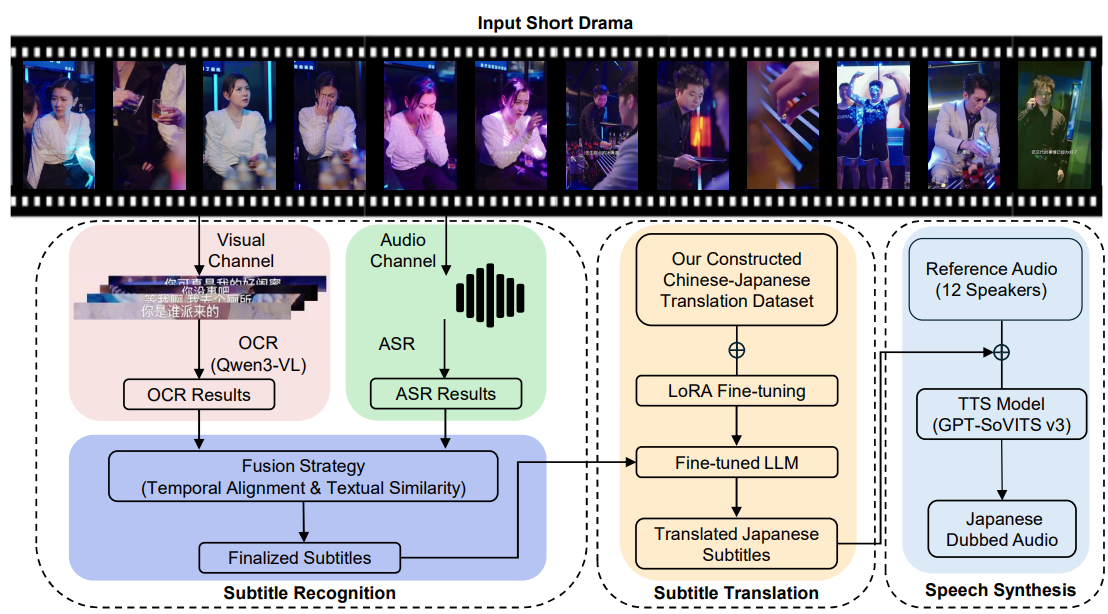
\includegraphics[width=\columnwidth]{fig_1_v2.png}
\caption{Architecture of the proposed end-to-end multimodal system: (1) subtitle recognition via parallel OCR (Qwen3-VL) and ASR (Whisper) with adaptive fusion; (2) translation using a LoRA fine-tuned Qwen3-VL; and (3) speech synthesis via zero-shot voice cloning. Stage~3 is new relative to the conference paper~\cite{an2026icassp}.}
\label{fig:system}
\end{figure}

\subsection{Subtitle Recognition}
\label{sec:recognition}

\subsubsection{Visual Channel: Frame-Level OCR}
Frames are sampled at a configurable rate (1\,fps for efficiency, 5\,fps for higher recall; Section~\ref{sec:fps_ablation}) and processed by Qwen3-VL~\cite{qwen3vl2025} with a structured prompt that outputs only the detected subtitle text (with a \texttt{``No subtitles''} fallback), minimising hallucination of logos and signage.

\subsubsection{Audio Channel: ASR with Timestamps}
Whisper~\cite{radford2023robust} transcribes the full audio track with word- and segment-level timestamps; trained on 680{,}000 hours of multilingual audio it covers conversational Chinese well, but is prone to phonetically plausible substitutions on rare proper nouns---precisely the errors the OCR channel corrects.

\subsubsection{Adaptive Multimodal Fusion}
\label{sec:fusion}

\paragraph{Notation}
Let $\mathcal{A}=\{a_i=(t_i^s,t_i^e,w_i,p_i)\}$ be the Whisper segments (start/end timestamps, text $w_i$, segment-level average log-probability $p_i$) and $\mathcal{O}=\{o_j=(\tau_j,c_j)\}$ the Qwen3-VL OCR detections (frame timestamp $\tau_j$, text $c_j$); $\mathrm{sim}(u,v)\in[0,1]$ is the RapidFuzz indel-edit character similarity.

\paragraph{Confidence-adaptive fusion}
Our fusion strategy leverages the complementary strengths of OCR (high precision for on-screen text, but no native temporal grounding) and ASR (fluent temporal segmentation, but phonetic substitution errors on rare proper nouns).
For each Whisper segment $a_i$ we (i) gather all OCR candidates whose frame timestamp falls within an expanded window $[t_i^s - \delta,\, t_i^e + \delta]$ with $\delta = 1.5$\,s, (ii) gate on the ASR log-probability $p_i$ relative to a confidence threshold $\theta_p$, and (iii) when ASR is uncertain, replace $w_i$ with the most similar OCR candidate provided that the similarity exceeds $\theta_s$.
The full procedure (Algorithm~1) is given in the Supplementary Material.
Both $\theta_p$ and $\theta_s$ are selected by a systematic grid search on a 20-episode validation subset (episodes 3--23, excluding episode 10); the search procedure and results are detailed in Section~\ref{sec:param_selection}, which selects $\theta_p = -0.2$ (nats) and $\theta_s = 80\%$.



This design is \emph{conservative} (confident ASR is never overridden, so non-subtitle on-screen text cannot intrude) and \emph{robust} (uncertain ASR is corrected only by a textually close OCR candidate, which empirically corresponds to phonetic proper-noun substitutions); it strictly beats the always-OCR/always-ASR extremes and matches a well-tuned static threshold while skipping OCR on confident segments (Section~\ref{sec:fusion_results}).

\subsection{Subtitle Translation}
\label{sec:translation}

\subsubsection{Context-Aware Translation}
A key design decision in our translation module is to process the entire subtitle sequence of an episode as a single translation task, rather than translating individual segments in isolation.
This holistic approach preserves dialogue coherence, pronoun referents, and narrative flow across the episode, all of which are critical for accurate subtitle translation.

\subsubsection{Model Selection and Fine-Tuning}
We adopt Qwen3-VL~\cite{qwen3vl2025} as our primary translation model, leveraging its strong Chinese--Japanese bilingual capabilities and its ability to optionally condition on video frame context.
We also evaluate Qwen2.5-3B, Qwen2.5-7B~\cite{yang2024qwen2}, and Qwen3-8B~\cite{qwen3_2025} as text-only translation baselines, and NLLB-200~\cite{nllb2022} and M2M-100 (1.2B)~\cite{fan2021beyond} as dedicated multilingual MT baselines.

For fine-tuning, we apply 4-bit quantization combined with LoRA~\cite{hu2022lora} to efficiently adapt the model parameters.
The LoRA configuration uses rank $r = 32$ and scaling factor $\alpha = 64$ for Qwen3-VL (optimized for the larger model capacity), and $r = 16$, $\alpha = 32$ for the text-only LLM fine-tunes (Qwen2.5-3B, Qwen3-8B).
LoRA adapters are applied to the query, key, value, output projection matrices, and the feed-forward gate, up, and down projection layers, to maximize adaptation scope.
Training is conducted using a 5-fold cross-validation scheme with random shuffled splitting (\texttt{KFold}, \texttt{shuffle=True}, \texttt{random\_state=42}) to ensure evaluation robustness on the limited 79-episode dataset; the same split is applied consistently to all models.
The primary Qwen3-VL model is trained for up to 20 epochs with early stopping (patience of 3 evaluations) at a learning rate of $5 \times 10^{-5}$ and an effective batch size of 4 (1 sample $\times$ 4 gradient accumulation steps); the text-only Qwen3-8B fine-tune uses a separately tuned schedule (up to 15 epochs, patience 5, learning rate $1 \times 10^{-4}$) at the same effective batch size.

\subsubsection{Multimodal Translation}
The fine-tuned translation models operate on text-only input (the fused subtitle sequence).
To assess the value of visual context, we additionally evaluate a multimodal variant in which representative video frames from each episode accompany the subtitle text, allowing the model to leverage visual information such as character appearance, scene type, and emotional context; this variant is studied as an ablation in Section~\ref{sec:ablation_context}.

\subsection{Speech Synthesis}
\label{sec:tts}

The final stage converts the translated Japanese into speech, using each of the 12 speakers' original Chinese audio as a timbre reference, and evaluates four TTS systems:
\textbf{GPT-SoVITS}~\cite{gptsovits2024} (v3, GPT acoustic model + SoVITS vocoder for reference-based cross-lingual cloning);
\textbf{F5-TTS}~\cite{chen2024f5tts} (flow-matching zero-shot synthesis);
\textbf{CosyVoice2-0.5B}~\cite{cosyvoice2_2024} (Alibaba's LLM-based flow-matching system with language tokens); and
\textbf{EdgeTTS}~\cite{edgetts2024} (Microsoft's API with a fixed Japanese voice and no cloning, an off-the-shelf fallback).
Each receives the Japanese text and, where applicable, a reference clip; outputs are scored by Whisper re-transcription.

%%
%% Experiments
%%
\section{Experiments}
\label{sec:experiments}

\subsection{Implementation Details}
All experiments are conducted on NVIDIA A100 SXM4 80\,GB GPUs running Ubuntu Linux.
The software environment uses Python~3.10 with PyTorch, the Hugging Face Transformers library, and PEFT for LoRA fine-tuning, with 4-bit weight quantization following QLoRA.
Video frame extraction is performed using OpenCV at the specified sampling rate.
For OCR, Qwen3-VL is deployed via a local vLLM inference service, which we found necessary to keep 5\,fps recognition tractable on a single GPU.
ASR is performed using the Whisper~medium checkpoint~\cite{radford2023robust}.
Translation metrics are computed using SacreBLEU~\cite{post2018sacrebleu} (BLEU and chrF++) with the standard \texttt{nrefs:1|case:mixed|tok:13a|smooth:exp|version:2.4.0} signature, and COMET via the \texttt{wmt22-comet-da} checkpoint.
TTS evaluation uses Whisper-medium to transcribe generated audio and \texttt{jiwer} to compute CER (character level, NFKC-normalised, punctuation stripped) and WER (over MeCab-tokenised text) against the Japanese reference.

\subsection{Evaluation Metrics}
\label{sec:metrics}

\textbf{Subtitle Recognition}: We report Character Error Rate (CER, lower is better), Character Accuracy (CharAcc, higher is better), BLEU~ (0--100 scale, higher is better), and chrF++~\cite{popovic2015chrf} (0--100, higher is better).
We also report a composite score defined as:
\begin{equation}
\text{Composite} = \frac{(1 - \text{CER}) + \text{CharAcc} + \frac{\text{BLEU}}{100} + \frac{\text{chrF++}}{100}}{4}
\label{eq:composite}
\end{equation}
which aggregates all four metrics into a single scalar for ranking.
The equal weighting is a presentational convenience; the headline fusion result (Table~\ref{tab:fusion}) holds for every constituent metric individually, so no conclusion depends on the specific weights.

\textbf{Subtitle Translation}: We report BLEU, chrF++~\cite{popovic2015chrf}, and COMET~\cite{rei2020comet} (0--1, higher is better).

\textbf{TTS}: We report Word Error Rate (WER, lower is better) and Character Error Rate (CER, lower is better), computed by transcribing the generated audio with Whisper and comparing against the reference Japanese text.

\subsection{Subtitle Recognition: Model Comparison}
\label{sec:ocr_comparison}

Recognition performance is summarised below (full per-model table in the Supplementary Material); all OCR results use temporal deduplication to avoid inflated CER from repeated frames.
At 1\,fps, the traditional \textbf{RapidOCR}~\cite{rapidocr2022} attains the best BLEU (86.3, CER 0.154) and \textbf{InternVL2-4B}~\cite{chen2024internvl} the best character accuracy (0.985, BLEU 83.5), showing that well-engineered traditional and VLM recognizers both excel on clean subtitle text.
\textbf{Qwen3-VL-4B}~\cite{qwen3vl2025} at 1\,fps (CER 0.402) trails them due to low frame recall, but at 5\,fps it leads on CER (0.086, CharAcc 0.982; Section~\ref{sec:fps_ablation}).
\textbf{TrOCR}~\cite{li2021trocr} (English-pretrained) fails on Chinese (BLEU 0.0), emitting hallucinated Latin tokens, and the general-purpose \textbf{Florence-2-large}~\cite{florence2_2024} scores far below task-specific models (CER 1.646)---confirming that language-appropriate, task-specific recognizers are essential for this domain.



\subsection{Frame Sampling Rate Ablation}
\label{sec:fps_ablation}

Short-drama dialogue changes 2--5 times per second, far exceeding 1\,fps coverage.
On episode \texttt{11.mp4}, detected characters (a recall proxy) rise from 411 at 1\,fps (27.7\% of the 5\,fps total) through 659 at 2\,fps (44.3\%) to 1{,}486 at 5\,fps (Supplementary Material), and correspondingly Qwen3-VL-4B's corpus CER drops from 0.402 (1\,fps) to 0.086 (5\,fps); we therefore use 5\,fps in production.
Competing methods are compared at 1\,fps because per-frame accuracy is rate-independent---the gain comes from capturing more frames, not higher per-frame fidelity---so 1\,fps reflects each model's intrinsic accuracy; a uniform 5\,fps VLM comparison, which also requires subtitle-line deduplication, is left to future work.



\subsection{Fusion Hyperparameter Selection}
\label{sec:param_selection}



The Supplementary Material reports the composite scores on the 20-episode validation subset (episodes 3--23, excluding episode 10) for a $10 \times 7$ grid over $\theta_p \in \{-1.5,\,-1.2,\,-1.0,\,-0.8,\,-0.6,\,-0.5,\,-0.4,\,-0.3,\,-0.2,\,0.0\}$ and $\theta_s \in \{30\%,\,40\%,\,50\%,\,60\%,\,70\%,\,80\%,\,90\%\}$ (representative rows and columns shown).
All configurations are evaluated in a consistent segment-joining text format to ensure fair comparison across parameter settings; absolute scores are not directly comparable to the production metrics in Table~\ref{tab:fusion}.
The search reveals two clear patterns.

First, $\theta_p$ must be set above $-0.8$ for any improvement over the no-replacement baseline (the flat upper region).
Analysis of the Whisper log-probability distribution on our corpus shows that avg\_logprob ranges from $-0.96$ to $-0.03$ (median $-0.30$) across 3,907 Whisper-generated segments (which may exceed the 3,692 ground-truth subtitle segments because Whisper also creates segments from non-subtitle speech), with only 1.6\% of segments falling below $-0.8$.
Consequently, $\theta_p \leq -0.8$ produces essentially zero OCR substitutions.
At $\theta_p = -0.2$, approximately 77.5\% of segments satisfy $p_i < \theta_p$ and enter the similarity check; at $\theta_p = -0.5$, only 13.2\% do.
The broad activation at $\theta_p = -0.2$ means the similarity gate $\theta_s$ becomes the primary filter, which explains the second pattern.

Second, within the active region, $\theta_s$ is the primary design choice: $\theta_s = 80\%$ (stricter matching) prevents false replacements from visually similar but semantically wrong OCR candidates, while $\theta_s \leq 30\%$ (permissive) over-replaces and introduces noise.
This finding is consistent with the degenerate threshold=0 case in the gating ablation (Supplementary Material).
The validation selects $\theta_p = -0.2$, $\theta_s = 80\%$, which we adopt throughout.
We additionally verify the sensitivity of the time tolerance parameter $\delta$ by evaluating $\delta \in \{0.5, 1.0, 1.5, 2.0\}$\,s with $\theta_p = -0.2$ and $\theta_s = 80\%$ fixed; the CER varies by less than 0.0001 across this range (0.162 in all cases), confirming that $\delta$ has negligible impact and that $\theta_s$ is the sole critical parameter once $\theta_p$ is set.

\subsection{Adaptive Multimodal Fusion}
\label{sec:fusion_results}

Table~\ref{tab:fusion} presents the results of the adaptive multimodal fusion strategy compared to using either modality in isolation; the Supplementary Material provides a threshold sensitivity ablation.
We evaluate three configurations in Table~\ref{tab:fusion}: (1) Qwen3-VL OCR only (without ASR timestamp anchors), (2) Whisper ASR only, and (3) our logprob-adaptive fusion.

The OCR-only configuration performs poorly (BLEU 4.44, CER 0.900) because the evaluation framework requires Whisper-format timestamped segments for alignment with the ground truth; without ASR providing temporal anchors, OCR outputs cannot be properly aligned to the reference subtitles.
Whisper alone achieves BLEU 81.32 and CER 0.249, confirming its strong baseline performance.
The Adaptive Fusion configuration improves over Whisper across all metrics: BLEU increases from 81.32 to 81.68, chrF++ improves substantially from 57.64 to 67.91, and CER decreases from 0.249 to 0.156.
The composite score improves by 0.079 (a relative gain of +10.8\%), primarily driven by the chrF++ improvement, which reflects successful correction of Whisper's character-level errors by OCR.

These results confirm that OCR effectively corrects Whisper's phonetically plausible but semantically incorrect substitutions---particularly for proper nouns---while ASR provides the temporal structure necessary for subtitle alignment.

\begin{table}[t]
\centering
\caption{Adaptive multimodal fusion results. Composite score defined in Eq.~\ref{eq:composite}. Best results in bold.}
\label{tab:fusion}
\resizebox{\columnwidth}{!}{%
\begin{tabular}{lccccc}
\toprule
\textbf{Configuration} & \textbf{BLEU}$\uparrow$ & \textbf{chrF++}$\uparrow$ & \textbf{CER}$\downarrow$ & \textbf{CharAcc}$\uparrow$ & \textbf{Comp.}$\uparrow$ \\
\midrule
OCR Only    & 4.44 & 9.29 & 0.900 & 0.100 & 0.084 \\
Whisper Only  & 81.32 & 57.64 & 0.249 & 0.783 & 0.731 \\
Adaptive Fusion (ours) & \textbf{81.68} & \textbf{67.91} & \textbf{0.156} & \textbf{0.899} & \textbf{0.810} \\
\bottomrule
\end{tabular}}
\end{table}



\textbf{Gating-rule ablation under a unified harness.}
To enable a like-for-like comparison between static thresholds and the adaptive gate---which the production pipeline does not permit post-hoc owing to its irreversible text-joining step---we re-evaluate every gating configuration inside a single harness: the same fusion implementation and the same corpus-level metrics used for the grid search (Section~\ref{sec:param_selection}), applied to all 79 episodes (Supplementary Material).
Three findings emerge.
First, both degenerate extremes are strictly sub-optimal: ``Always Replace'' collapses catastrophically (BLEU 0.51) because unconditional substitution adopts hallucinated or empty OCR detections whenever any candidate falls in the time window, and ``Never Replace'' (ASR only) forfeits all correction benefits (composite 0.8066 vs.\ 0.8094 for the best gated variant).
Second, within the gated regime the similarity threshold is the primary driver, with a shallow optimum around $\theta_s \in [40, 80]$ (composite 0.8091--0.8094).
Third, the adaptive operating point ($\theta_p{=}-0.2$, $\theta_s{=}80$) performs on par with the best static threshold (composite 0.8091 vs.\ 0.8094; BLEU 81.60 vs.\ 81.61 for static $\theta_s{=}80$)---a statistical tie.
We therefore do \emph{not} claim an accuracy advantage for the log-probability gate over a well-tuned static threshold; its practical value is that it (i) exempts the $\sim$22\% of segments where ASR is already confident from OCR consultation, reducing fusion-stage computation without sacrificing accuracy, and (ii) provides a principled, data-driven way to select the operating point via the grid search of Section~\ref{sec:param_selection} rather than manual threshold tuning.
The system-level benefit of fusion over the ASR-only production baseline ($+10.8\%$ composite) is established independently in Table~\ref{tab:fusion}.

\subsection{Subtitle Translation: Model Comparison}
\label{sec:translation_results}

Table~\ref{tab:translation} reports translation results; all BLEU/chrF\texttt{++} use a standardised \texttt{strip\_nums}+\texttt{ja-mecab} protocol and are evaluated at the document level (full-episode input vs.\ full-episode reference), which avoids segment-alignment artefacts and matches the fine-tuned model's training.
Fine-tuned \textbf{Qwen3-VL-4B} reaches BLEU $15.70\pm4.42$ (5-fold CV), $+32\%$ over its zero-shot baseline (11.93), aided by full-episode context, an $r{=}32/\alpha{=}64$ LoRA, and a low learning rate; it is statistically comparable to zero-shot \textbf{Qwen3-8B} (17.46, $p=0.453$) at half the parameters.
Fine-tuning \textbf{Qwen3-8B} reaches BLEU $19.69\pm2.49$ / COMET $0.860$ ($+2.23$ over its zero-shot), and fine-tuning the strongest baseline \textbf{Gemma-4-12B} reaches $30.75\pm1.84$ / chrF\texttt{++} $30.63$ ($+4.51$ over its zero-shot 26.24), the best overall---so domain LoRA fine-tuning helps at every scale (4B $+32\%$, 8B $+13\%$, 12B $+17\%$).
Gemma's COMET is essentially unchanged by fine-tuning ($0.890$ vs.\ $0.892$) despite the large surface-metric gain, suggesting fine-tuning mainly aligns lexical choice and register rather than meaning (or reflects COMET's upper-range compression); the practical upshot is a quality--cost spectrum from a consumer-GPU 4B fine-tune to the best-quality 12B.
We make no single-model state-of-the-art claim: the translation-stage contribution is this systematic cross-scale fine-tuning demonstration on a previously unstudied domain, while the pipeline, dataset, and fusion are the system-level contributions.
Among the remaining baselines, \textbf{Qwen2.5-3B} fine-tuning gains $+9.52$ BLEU (ZS 3.58 $\to$ FT 13.10; the low ZS reflects a speaker-tag formatting artefact, ZS COMET 0.71), whereas dedicated MT models \textbf{M2M-100} (6.33) and \textbf{NLLB-200} (2.97) transfer poorly to colloquial speaker-tagged subtitles; per-baseline analysis continues in Section~\ref{sec:discussion_translation}.

\begin{table}[t]
\centering
\caption{Subtitle translation results. FT$^{\star}$ = LoRA fine-tuned (5-fold CV mean$\pm$std); ZS = zero-shot; +V = with visual frames. BLEU/chrF\texttt{++} use \texttt{strip\_nums}+\texttt{ja-mecab}. Bold: best per column. $^{\ddagger}$Qwen2.5-3B ZS prepends phonetic speaker tags (COMET 0.71 stays high); $^{\S}$Qwen3.5-9B chain-of-thought exhausted the token budget before emitting Japanese.}
\label{tab:translation}
\resizebox{\columnwidth}{!}{%
\begin{tabular}{llccc}
\toprule
\textbf{Model} & \textbf{Set.} & \textbf{BLEU}$\uparrow$ & \textbf{chrF++}$\uparrow$ & \textbf{COMET}$\uparrow$ \\
\midrule
Gemma-4-12B~\cite{gemma2025}     & FT$^{\star}$ & \textbf{30.75}$_{\pm1.84}$ & \textbf{30.63}$_{\pm2.01}$ & $0.890$ \\
Gemma-4-12B~\cite{gemma2025}     & ZS+V & 26.27 & 28.65 & \textbf{0.892} \\
Qwen3-8B~\cite{qwen3_2025}       & FT$^{\star}$ & 19.69$_{\pm2.49}$ & 23.41$_{\pm1.28}$ & $0.860$ \\
Qwen3-8B~\cite{qwen3_2025}       & ZS   & 17.46 & 21.03 & 0.864 \\
Qwen3-VL-4B~\cite{qwen3vl2025}   & FT$^{\star}$ & $15.70_{\pm4.42}$ & $20.78_{\pm2.81}$ & $0.843$ \\
InternVL3-8B~\cite{chen2024internvl} & ZS+V & 13.65 & 17.76 & 0.788 \\
Qwen2.5-3B~\cite{yang2024qwen2}  & FT   & 13.10 & 16.94 & 0.644 \\
Qwen2.5-7B~\cite{yang2024qwen2}  & ZS   & 12.89 & 18.31 & 0.829 \\
Qwen3-VL-4B~\cite{qwen3vl2025}   & ZS   & 11.93 & 17.72 & 0.810 \\
M2M-100~\cite{fan2021beyond}     & ZS   &  6.33 & 11.28 & 0.515 \\
SeamlessM4T-v2~\cite{seamless2023} & ZS &  5.67 & 12.13 & 0.497 \\
Qwen2.5-3B~\cite{yang2024qwen2}  & ZS   & 3.58$^{\ddagger}$ & 11.64 & 0.713 \\
Qwen3.5-9B~\cite{qwen35_2025}    & ZS+V & 3.49$^{\S}$ & 11.79 & 0.420 \\
NLLB-200~\cite{nllb2022}         & ZS   &  2.97 &  6.19 & 0.378 \\
\bottomrule
\end{tabular}}
\end{table}



\subsection{Text-to-Speech Comparison}
\label{sec:tts_results}

The TTS evaluation (WER, CER, Resemblyzer speaker similarity; full table in the Supplementary Material) is summarised here.
Intelligibility metrics are computed by transcribing the synthesised audio with Whisper-medium (\texttt{language=ja}); reference and hypothesis are NFKC-normalised with punctuation stripped, CER is computed at the character level, and WER is computed over MeCab-tokenised text (the \texttt{ja-mecab} tokeniser), since whitespace-based WER is ill-defined for unsegmented Japanese.
We use Resemblyzer~\cite{resemblyzer2020} as a lightweight, fully offline speaker encoder that requires no task-specific fine-tuning; it computes a 256-dimensional $d$-vector from raw waveform and has been widely adopted as an automatic proxy for speaker identity in zero-shot TTS evaluation~\cite{chen2024f5tts,cosyvoice2_2024}.
We acknowledge that automatic Spk-Sim is a proxy and may not fully align with human-perceived voice similarity, and we treat CER as the primary intelligibility metric.
\textbf{EdgeTTS}~\cite{edgetts2024}, a commercial system with a fixed professionally tuned Japanese voice, is the most intelligible overall (CER 0.030, WER 0.056), as expected for a production service that performs no voice cloning.
\textbf{GPT-SoVITS v3}~\cite{gptsovits2024} is by far the most intelligible of the three voice-cloning systems (CER 0.215, median 0.091)---roughly $5\times$ better than F5-TTS and over $20\times$ better than CosyVoice2 on mean CER---while its speaker similarity of 0.722 indicates strong voice identity preservation under cross-lingual cloning.
GPT-SoVITS produced usable synthesis for 6 of the 12 speakers, so its average is computed over those 6; restricting all systems to this common 6-speaker subset leaves the ranking and gaps essentially unchanged (GPT-SoVITS CER 0.215, F5-TTS 1.269, CosyVoice2 6.514), confirming the comparison is not an artefact of differing speaker coverage.
\textbf{F5-TTS}~\cite{chen2024f5tts} attains the highest speaker similarity (0.729) but produces largely unintelligible cross-lingual output (CER 1.152): transcriptions frequently contain garbled multilingual fragments, indicating that it preserves timbre but fails to produce fluent Japanese from Chinese references.
\textbf{CosyVoice2-0.5B}~\cite{cosyvoice2_2024} exhibits the weakest intelligibility (mean CER 4.603, median 1.0); inspection of the transcriptions reveals a degenerate repetition failure mode on a subset of inputs, where the model emits long vowel loops instead of speech---likely a capacity limitation of the 0.5B variant under cross-lingual prompting.
The dissociation between intelligibility and speaker similarity highlights an important trade-off: F5-TTS captures timbre marginally better than GPT-SoVITS (0.729 vs.\ 0.722) but at a catastrophic intelligibility cost.

Overall, the intelligibility ranking is EdgeTTS $>$ GPT-SoVITS $\gg$ F5-TTS $>$ CosyVoice2, while the speaker-similarity ranking among cloning systems is F5-TTS $\approx$ GPT-SoVITS $>$ CosyVoice2; GPT-SoVITS offers the best overall balance and is the only cloning system with usable intelligibility.

Regarding evaluation methodology: we follow the automatic evaluation protocol adopted in the F5-TTS~\cite{chen2024f5tts} and CosyVoice2~\cite{cosyvoice2_2024} papers, where ASR-based intelligibility and speaker-embedding cosine similarity jointly characterise zero-shot TTS quality.
To validate the automatic ranking perceptually, we additionally conducted a blind human listening study, reported in Section~\ref{sec:tts_human}; the two evaluations agree on the system ordering.



\subsubsection{Human Listening Study}
\label{sec:tts_human}

We complement the automatic metrics with a blind listening study: five JLPT-N1 raters scored 8 speaker--sentence items per system (160 naturalness ratings) on a 5-point MOS scale under randomised blind codes, and chose the clip most similar to the reference (full protocol and per-system table in the Supplementary Material).



GPT-SoVITS (MOS $3.08\pm1.14$) is statistically indistinguishable from commercial EdgeTTS ($3.12\pm1.14$; Wilcoxon paired by rater--item, $z=-0.09$, $p=0.93$) and both far exceed F5-TTS ($1.80$) and CosyVoice2 ($1.52$; both $p<0.001$)---matching a fixed commercial voice while performing zero-shot cloning is a strong result.
On perceived similarity GPT-SoVITS dominates (45\% of votes vs.\ 15\% F5-TTS, 5\% CosyVoice2; EdgeTTS 0\%); although F5-TTS has marginally higher \emph{automatic} similarity (0.729 vs.\ 0.722; Supplementary Material), raters preferred GPT-SoVITS 3:1, showing embedding similarity alone misses perceptual identity, and the 35\% ``none'' votes reflect the difficulty of cross-lingual cloning from short references.
Inter-rater reliability is ICC(2,1)=0.30 / ICC(2,$k$)=0.68 (Krippendorff's ordinal $\alpha$=0.31), typical for small MOS panels.
The human study thus corroborates the automatic ranking: GPT-SoVITS uniquely combines commercial-grade naturalness with effective cloning.

\subsection{Ablation Studies}
\label{sec:ablation}

\subsubsection{Translation Context: Visual vs.\ Text-Only}
\label{sec:ablation_context}

To quantify the benefit of visual context for translation, we compare two variants of Qwen3-VL-based translation:
(1) \textit{Text-only}: the model receives only the OCR-extracted Chinese subtitle text as input, and
(2) \textit{Multimodal}: the model receives both the subtitle text and representative video frames from the episode.

In the \emph{zero-shot} setting (Supplementary Material), the multimodal variant achieves BLEU 13.44 vs.\ 10.09 for text-only---a $+3.35$ BLEU gain.
This demonstrates that visual context provides meaningful information when the model is not adapted to the domain, likely by disambiguating character identities, emotional tone, and scene type that is otherwise lost in the subtitle text alone.

This benefit does \emph{not}, however, carry over to fine-tuning.
We fine-tuned Qwen3-VL-4B with four video frames per episode supplied during both training and inference, under the identical 5-fold protocol used for the text-only fine-tune (FT+V; per-fold results in the Supplementary Material).
The multimodal fine-tune achieves BLEU $15.58\pm6.49$ / chrF\texttt{++} $21.02\pm3.34$ / COMET $0.846\pm0.039$, statistically indistinguishable in mean from the text-only fine-tune ($15.70\pm4.42$ / $20.78\pm2.81$ / $0.843\pm0.026$; paired $t$-test on the five folds $t=-0.04$, $p=0.97$) but with markedly higher cross-fold variance (BLEU std $6.49$ vs.\ $4.42$; per-fold differences range from $-6.2$ to $+9.2$ BLEU).
We attribute this to redundancy and capacity: once LoRA adapts the model to the domain, text already carries most of the disambiguating context, while extra visual tokens consume limited adapter capacity and inject episode-specific noise, destabilising training on the 63-episode folds.
Visual grounding thus helps a non-adapted model but is redundant under fine-tuning, so the released pipeline fine-tunes on text.



\subsubsection{TTS Reference Audio Duration}
\label{sec:ablation_tts}

Zero-shot cloning quality depends on the reference clip.
Comparing F5-TTS under $\sim$3\,s vs.\ $\sim$10\,s references, speaker similarity improves $0.64\to0.71$ (Supplementary Material); we therefore recommend at least 8--10\,s of clean reference audio per speaker.



\subsection{Computational Cost and Efficiency}
For deployability we profile each stage on one A100 (80\,GB): Whisper-medium RTF $\approx0.08$, vLLM-served Qwen3-VL-4B OCR RTF $\approx0.5$ (1\,fps)/$\approx2.4$ (5\,fps) with a frame cache cutting re-runs by ${>}98\%$, LoRA translation 6--10\,s/episode, and GPT-SoVITS synthesis $\approx1.4\times$ output duration---an end-to-end $\approx3$--$4\times$ real-time factor suited to offline batch localization (full breakdown in the Supplementary Material).

%%
%% Discussion
%%
\section{Discussion}
\label{sec:discussion}

\subsection{Analysis of Recognition Results}
Frame sampling rate is the dominant recognition factor: 1\,fps captures only 27.7\% of subtitle content, and raising it to 5\,fps cuts Qwen3-VL-4B CER five-fold ($0.402\to0.086$), a trade-off well suited to offline processing.
The adaptive fusion resolves the complementary failure modes of OCR (weak temporal alignment) and ASR (phonetic proper-noun substitution); its $+10.8\%$ composite gain is concentrated in chrF\texttt{++} ($+10.3$), indicating mostly character-level corrections.

\textbf{Fusion error-type analysis.}
A jieba POS-tagged word-level diff between ASR-only and fused outputs (all 79 episodes; Supplementary Material) shows that of 227 substitutions, proper nouns (13.2\% of changes) are corrected toward the ground truth at a 60.0\% rate, slightly above common vocabulary (59.1\%)---the fusion makes linguistically targeted corrections of rare entities, e.g.\ \emph{李福}(nr)$\to$\emph{礼服}(n) (a homophonic common noun mis-tagged as a name) and \emph{陆少庆}$\to$\emph{陆少} (a spurious appended character).



\subsection{Analysis of Translation Results}
\label{sec:discussion_translation}
Fine-tuned Qwen3-VL-4B improves over its zero-shot baseline by $+32\%$ BLEU ($15.70\pm4.42$ vs.\ 11.93), with consistent chrF\texttt{++} (20.78 vs.\ 17.72) and COMET (0.843 vs.\ 0.810) gains; the $\pm4.42$ cross-fold spread reflects genuine domain heterogeneity.
The fine-tuned model beats its zero-shot counterpart on Folds 0/1/3 but loses on the two highest-OOV folds (Fold~2 and Fold~4 have 36.3\% and 35.7\% word-level OOV vs.\ 33.0--33.1\% elsewhere), where novel character names and slang favour the base model's broader pre-training.
Scaling LoRA to 8B mitigates this (Fold~2 17.53, Fold~4 19.51 vs.\ 9.58/12.94 at 4B), and the larger zero-shot models show low cross-fold variance ($\pm0.98$ Gemma, $\pm1.00$ Qwen3-8B); augmenting training with multiple series to reduce OOV is a clear future direction.
The large Qwen2.5-3B gain (ZS 3.58 $\to$ FT 13.10) partly reflects a zero-shot speaker-tag artefact, yet the fine-tuned 3B still exceeds the larger Qwen2.5-7B zero-shot (12.89).
Visual context adds $+3.35$ BLEU in zero-shot, motivating tighter multimodal integration.

\textbf{Qualitative analysis.}
The Supplementary Material lists two characteristic error patterns (qualitative examples).
In Example~A, the source phrase \textit{看来我们挺有缘} contains the culturally loaded term 缘 (a predestined fate or karmic connection between people).
The fine-tuned model correctly maps it to the Japanese 縁 (\textit{en})---preserving both meaning and cultural nuance---whereas the zero-shot baseline substitutes 運 (\textit{un}, ``luck''), losing the relational concept.
In Example~B, from Fold~2 (word OOV rate 36.3\%), the source 拜托 (``come on'' / ``please'') triggers a domain-specific hallucination in the fine-tuned model: it generates a sentence about the drama character ``White''---a fashion designer encountered in the training episodes---despite the source being a short exclamation.
This is a direct symptom of the OOV-driven generalisation failure discussed above: the model over-fits to co-occurring characters in training episodes and mis-fires on validation episodes with different character distributions.



Across baselines (Table~\ref{tab:translation}), \textbf{Gemma-4-12B} leads in both regimes (zero-shot 26.27 BLEU / 0.8917 COMET; fine-tuned 30.75 / chrF\texttt{++} 30.63, best overall).
Our fine-tuned 4B (15.70, COMET 0.843) trails it but uses one-third the parameters under stricter cross-validation, while \textbf{Qwen3-8B} zero-shot (17.46, 0.864) edges it on BLEU at twice the size.
InternVL3-8B (13.65) underperforms at comparable scale, and Qwen3.5-9B (3.49) collapses because chain-of-thought exhausts the token budget before emitting Japanese; M2M-100 (6.33) and SeamlessM4T-v2 (5.67) confirm dedicated MT transfers poorly to colloquial speaker-tagged subtitles.
Overall the 4B fine-tune beats 9 of 11 zero-shot baselines, trailing only the larger Gemma-4-12B and Qwen3-8B.

\textbf{Statistical significance.}
Paired $t$-tests over the five folds confirm the Gemma-4-12B-ZS gap is significant ($t=-4.40$, $p=0.012$) while the Qwen3-8B-ZS gap is not ($t=-0.83$, $p=0.453$); Wilcoxon tests ($p=0.063$, $0.813$) and fold-level bootstrap CIs agree (Supplementary Material).

\textbf{Cross-stage error propagation.}
Recognition errors in stage~1 propagate to translation.
Simulating recognition noise (random character substitution in the oracle source, then translating with the fold-0 LoRA model) gives an approximately linear CER--BLEU relation: at the ASR-only point (CER 0.249) translation BLEU falls to 3.5 vs.\ 13.1 for clean source, while the adaptive fusion (CER 0.156) recovers $\approx\textbf{+2.2}$ BLEU.
A direct end-to-end evaluation on the 16 fold-0 episodes (document level) confirms this: fusion reaches chrF\texttt{++} 13.56 vs.\ 11.32 for ASR-only, recovering \textbf{$+2.24$} points (61\% of the oracle ceiling 14.97).
Document-level BLEU for ASR-only is 0.00 because propagated proper-noun errors eliminate all episode-level 4-gram overlap---a genuine linguistic effect, hence chrF\texttt{++} is the primary metric here.





\subsection{Qualitative Error Analysis}
A manual inspection of 100 held-out segments groups remaining errors into four orthogonal categories---proper-noun substitution (38\%), empty-frame OCR over-trigger (22\%), translation register mismatch (24\%), and TTS prosodic flattening (16\%)---so stage-specific improvements should be additive (details in the Supplementary Material).

\subsection{Limitations}
First, our corpus is a single short-drama series, which may limit cross-genre generalizability; the genre-intrinsic traits (fast colloquial dialogue, dense proper nouns, fragmented unpunctuated segments) make it a representative but not exhaustive benchmark, and the per-fold OOV patterns of Section~\ref{sec:discussion_translation} may differ across genres---so multi-series training and cross-genre evaluation are key future work.
Second, the human listening study is small ($n=5$) and uses JLPT-N1 non-native rather than native Japanese raters (single-rating ICC(2,1)$=0.30$); a larger native panel would tighten the estimates.
Third, the pipeline operates offline; real-time processing would require further OCR-stage optimization.

%%
%% Conclusion
%%
\section{Conclusion}
\label{sec:conclusion}

This paper presents a comprehensive end-to-end multimodal system for subtitle recognition and Chinese--Japanese translation in short dramas.
Our system integrates multiple state-of-the-art components: Qwen3-VL for frame-level OCR, Whisper for timestamp-anchored ASR, an adaptive confidence-based fusion strategy, LoRA fine-tuned Qwen3-VL for context-aware translation, and neural TTS for Japanese speech synthesis.

Our key findings: 5\,fps sampling is essential for OCR recall (CER $0.402\to0.086$); the confidence-gated fusion improves the composite recognition score by $+10.8\%$ over ASR-only while matching a well-tuned static threshold and skipping confident segments; domain LoRA fine-tuning helps at every scale (BLEU 15.70 at 4B, 19.69 at 8B, 30.75 at 12B), with visual context helping zero-shot but not fine-tuning; and GPT-SoVITS is the only TTS system combining commercial-grade naturalness (MOS 3.08, tied with EdgeTTS) with effective cloning (45\% of human similarity votes). The fusion's recognition gains propagate downstream to $+2.24$ chrF\texttt{++}.
Future work will extend the corpus to multiple series and genres, explore learned multimodal fusion and confidence estimators, and optimise the pipeline for low-latency deployment.

%%
%% Reproducibility, Data Availability, Ethics
%%
\section*{Reproducibility Statement}
We provide full details necessary to reproduce our experiments.
Section~\ref{sec:method} specifies the model variants, prompt templates, and fusion thresholds; Section~\ref{sec:translation} reports LoRA hyperparameters, optimizer settings, batch size, and training schedule; Section~\ref{sec:experiments} reports hardware, software stack, and evaluation toolchain (SacreBLEU signature, COMET checkpoint, jiwer for WER/CER).
The 5-fold cross-validation split protocol and seeds are described in Section~\ref{sec:translation_results}.
Upon publication, we will release the inference and training scripts for the full pipeline together with the configuration files used for every reported number.

\section*{Data Availability}
The Chinese--Japanese short-drama corpus used in this work was provided by a commercial entertainment company under a research-use agreement that prohibits public redistribution of the underlying video, audio, and subtitle files.
We will release a fully redacted metadata package (per-episode statistics, segment counts, fold assignments, and evaluation hashes) sufficient to reproduce our split protocol and to align future runs that obtain the source material via a comparable industry agreement.
Synthetic example outputs (translation pairs and short anonymized synthesis clips) will be released for qualitative inspection.

\section*{Ethics Statement}
The dataset was collected from a single commercial short-drama series with explicit permission from the rights holder for research use; performers in the source material are professional actors who consented to broadcast distribution.
Human annotators (Chinese subtitle reviewers and native Japanese translators) participated voluntarily and were compensated.
Our zero-shot voice cloning experiments use the original actors' voices solely as a reference for cross-lingual dubbing of \emph{the same characters' lines} from the same series, which mirrors the licensed downstream use; the released synthesis examples will be limited to short, content-neutral lines and clearly labelled as synthetic.
We caution that zero-shot voice cloning carries general misuse risk, and we therefore do not release reference-audio--to--cloned-voice mappings for the speakers.

%%
%% Acknowledgment
%%
\section*{Acknowledgment}
This work was supported by the Postdoctoral Fellowship Program for Overseas Talent Introduction, Ministry of Education of China.
The authors thank the commercial entertainment company that provided the short-drama dataset for research purposes, and the native Japanese researchers who contributed subtitle translations.

%%
%% Bibliography
%%
\bibliographystyle{IEEEtran}
\bibliography{refs}

%%
%% Author Biographies
%% Omitted from the initial submission to meet the 10-page limit; they do not
%% count toward the page limit and will be reinstated for the camera-ready
%% version. Change the guard below from false to true to re-enable them.
%%
\iffalse
\pagebreak
\begin{IEEEbiographynophoto}{Qiming Bao}
received the Ph.D. degree from the University of Auckland, Auckland, New Zealand.
He is currently an AI Researcher at the University of Auckland.
His research interests include multimodal large language models, vision--language understanding, neural machine translation, and end-to-end multimedia processing systems.
He is a joint first author of this work.
\end{IEEEbiographynophoto}

\begin{IEEEbiographynophoto}{Jing An}
received the Ph.D. degree from Tohoku University, Sendai, Japan, in 2018.
She is currently an Assistant Professor with the School of AI and Language Sciences, Beijing International Studies University, Beijing, China.
Her research interests lie at the intersection of multimedia information processing and language science, with a focus on multimodal subtitle localization and Chinese--Japanese language technology.
She is a joint first author and corresponding author of this work.
\end{IEEEbiographynophoto}

\begin{IEEEbiographynophoto}{Rui-Yang Ju}
is currently pursuing the Ph.D. degree at the Graduate School of Informatics, Kyoto University, Kyoto, Japan.
His research interests include computer vision and deep learning, with an emphasis on efficient neural network design for multimedia applications.
\end{IEEEbiographynophoto}

\begin{IEEEbiographynophoto}{Haofei Chang}
is currently an undergraduate student at the School of Information, Renmin University of China, Beijing, China.
His research interests include natural language processing and information extraction.
\end{IEEEbiographynophoto}

\begin{IEEEbiographynophoto}{Jinhua Su}
received the Ph.D. degree in Statistics from Renmin University of China, Beijing, China.
He is currently the CEO of Simashuhui Ltd., Beijing, China.
His research interests include subtitle translation and automatic speech recognition.
\end{IEEEbiographynophoto}

\begin{IEEEbiographynophoto}{Yanbing Bai}
received the Ph.D. degree from Tohoku University, Sendai, Japan, in 2017.
She is currently an Assistant Professor with the Center for Applied Statistics, School of Statistics, Renmin University of China, Beijing, China.
Her research interests include computer vision and large language models.
She is a corresponding author of this work.
\end{IEEEbiographynophoto}

\begin{IEEEbiographynophoto}{Xin Qu}
is currently a Professor with the School of AI and Language Sciences, Beijing International Studies University, Beijing, China.
Her research interests include computational linguistics and machine translation.
\end{IEEEbiographynophoto}

\begin{IEEEbiographynophoto}{Michael Witbrock}
received the Ph.D. degree in computer science from Carnegie Mellon University, Pittsburgh, PA, USA.
He is currently a Professor with the School of Computer Science, University of Auckland, Auckland, New Zealand, where he directs the Strong AI Lab (SAIL) within the Natural, Artificial and Organisational Intelligence Institute (NAOI).
His research interests lie at the intersection of machine learning, automated reasoning, and natural language understanding, with an emphasis on the beneficial societal impact of increasingly capable AI.
\end{IEEEbiographynophoto}
\fi

\end{document}
